

% Dies ist die Preambel
% \documentclass[12pt,a4paper,bibtotoc, twoside, cleardoublepage=empty]{article} % twoside
\documentclass[12pt,a4paper,bibtotoc, cleardoublepage=empty]{article}  % oneside centered



% das ist Standard - nie ohne aus dem Haus gehen
\usepackage[german]{babel}
% Biber!!!!!!!!!!!!!!!!!!


\usepackage{ebgaramond}

\usepackage{typearea}
\usepackage[style=authortitle]{biblatex}
\usepackage[babel,german=guillemets]{csquotes}
\bibliography{lit/literatur}



\usepackage[onehalfspacing]{setspace}

\usepackage{tabularx} % in the preamble

% Fu�noten auch in �berschriften
\usepackage[stable]{footmisc}

% Bilder
\usepackage{graphicx}
\graphicspath{ {../img/} } 
\usepackage{float} 

% Seitenraender 
\usepackage{geometry}

%\geometry{a4paper, top=20mm, left=35mm, right=20mm, bottom=20mm,headsep=12mm, footskip=12mm} % twoside
\geometry{a4paper, top=20mm, left=20mm, right=20mm, bottom=20mm,headsep=12mm, footskip=12mm} % oneside centered


%\usepackage{natbib}


%Hinweisbox
\usepackage{calc}
\usepackage{hhline} 
\usepackage{multirow} 
\usepackage{xcolor}
\usepackage{colortbl}
\usepackage{graphicx}

\newlength{\iconwidth}
\setlength{\iconwidth}{1cm}

\definecolor{boxheadcol}{gray}{.6}
\definecolor{boxcol}{gray}{.9}

\newenvironment{displaybox}[2]{%
  \begin{center}
    \setlength\arrayrulewidth{0.75pt}%
    \arrayrulecolor{white}%
    \renewcommand{\arraystretch}{1.3}%
    \begin{tabular}{p{\iconwidth}p{\linewidth-4\tabcolsep-\iconwidth}}
      \multirow{2}{*}{#2}&\cellcolor{boxheadcol}\textbf{\sffamily\color{white}#1} \\%
      \hhline{~-}%
      &\cellcolor{boxcol}%
}{%
      \\
    \end{tabular}
  \end{center}%
}


\newenvironment{Tipp}{%
\begin{displaybox}{Tipp}{
\includegraphics[width=\iconwidth]{../img/com/icon-tipp}}}%
{\end{displaybox}}

\newenvironment{Hinweis}{%
\begin{displaybox}{Hinweis}{
\includegraphics[width=\iconwidth]{../img/com/icon-hinweis}}}%
{\end{displaybox}}
%Hinweisbox ende

% Standart Kopfzeile 
\pagestyle{headings}
  
% Referenzen

\usepackage{hyperref}
\hypersetup{
  colorlinks=true,
  linkcolor=black,
  urlcolor=blue,
  pdfborder={0 0 0}
}

% Mit Mausklick zum Ziel
\usepackage{nameref}
% URLs
\usepackage{url} 



% Umlaute:
% Immer nur einen inputenc verwenden, sonst Fehler!
% Linux
% \usepackage[latin1]{inputenc} 
% Windows
\usepackage[utf8]{inputenc}

% Umlaute auch in der PDF
\usepackage[T1]{fontenc}

% Fuer jede Section eine neue Seite
\let\stdsection\section
\renewcommand\section{\newpage\stdsection}

% Fuer jede SubSection eine neue Seite
%\let\stdsubsection\subsection
%\renewcommand\subsection{\newpage\stdsubsection}

%\usepackage{natbib}	% Literaturverzeichnis

% \usepackage{skull}	% alles hat ein Ende

\usepackage{color}	% bring Farbe ins Spiel
% Fuer Codebeispiele
\definecolor{DarkPurple}{rgb}{0.4,0.1,0.4}
\definecolor{DarkCyan}{rgb}{0.0,0.5,0.4}
\definecolor{LightLime}{rgb}{0.4,0.6,0.5}
\definecolor{Blue}{rgb}{0.0,0.0,1.0}

\definecolor{forestgreen}{RGB}{34,139,34}
\definecolor{orangered}{RGB}{239,134,64}
\definecolor{darkblue}{rgb}{0.0,0.0,0.6}
\definecolor{gray}{rgb}{0.4,0.4,0.4}

% sch?nere Serifenfonts
\usepackage{times}		
\usepackage{lmodern}
	
% deutsche Abs?tze
\parskip2ex		% Absatzabsstand	
\parindent0ex		% Absatzeinzug

% keine Hurenkinder und Schusterjungen
\clubpenalty=10000
\widowpenalty=10000

% Fuer mehr Codeschnipsel Funktionen
\usepackage{moreverb}

\usepackage{listings}

% f?r Java-Bezeichner und -Keywords im Flie?text
\newcommand{\code}[1]{\small\lstinline[style=InlineJava]!#1!\normalsize}
%\newcommand{\code}[1]{\scriptsize\texttt{#1}\normalsize}

% fuer Listings mit Eintrag im Inhaltsverzeichnis
%\newcommand{\newlisting}[2]{
%\subsubsection*{Listing \ref{lst:#1}: #2}
%\addcontentsline{toc}{subsubsection}{\ref{lst:#1}. #2}}

\let\underscore\_
\newcommand{\myunderscore}{\renewcommand{\_}{\underscore\hspace{0pt}}}
%Issue the changed underscore command to the whole document.
\myunderscore

\lstdefinestyle{Java}
{
language=Java,
numberfirstline,
numberstyle=\tiny\sffamily,
tabsize=5,
captionpos=b,
aboveskip=1em,
belowskip=1em,
columns=flexible,
xleftmargin=2em,
xrightmargin=1em,
frame=single,
frameround=tttt,
commentstyle=\itshape\color{LightLime},
keywordstyle=\bfseries\color{DarkPurple},
basicstyle=\footnotesize\ttfamily,
stringstyle=\color{Blue},
showstringspaces=false,
}

\lstdefinestyle{XML} {
    language=XML,
    extendedchars=true, 
    breaklines=true,
    breakatwhitespace=true,
    emph={},
    emphstyle=\color{red},
    basicstyle=\ttfamily,
    columns=fullflexible,
    commentstyle=\color{gray}\upshape,
    morestring=[b]",
    morecomment=[s]{<?}{?>},
    morecomment=[s][\color{forestgreen}]{<!--}{-->},
    keywordstyle=\color{orangered},
    stringstyle=\ttfamily\color{black}\normalfont,
    tagstyle=\color{darkblue}\bf,
    morekeywords={attribute,xmlns,version,type,release},
}




\lstnewenvironment{javalisting}[1][]
{
	\lstset{language=Java, 
					 style=Java
	}
}
{}

\newenvironment{javalistingfigure}
{
\begin{figure}
\begin{javalisting}
}
{
\end{javalisting}
	\caption{asasas}
	\label{fig:javalisting}
\end{figure}
}


%\lstnewenvironment{javalisting}
%{
%\begin{center}
	%\begin{figure}

%		\begin{lstlisting}[style=Java]
		
		%		public class UserSession implements Serializable{}

%}
%{
%		\end{lstlisting} 

		%\caption{dsdsds}
		%\label{fig:sddsdsds}
		
	%\end{figure}
%\end{center}
%}

% Strikeout
\usepackage{ulem}

% Zeilenumbruch Bib
\renewcommand*{\labelnamepunct}{\newunitpunct\par}

\usepackage{chngcntr}
\counterwithin{figure}{section}

\begin{document}

%
%%% SIMPLE TITLE

%\frontmatter
\pagestyle{empty}
\clearpage

\newcommand*{\titleUL}{\begingroup% Hochschule Harz
\begin{center}

%\rule{\textwidth}{0.25pt}\par
% -- LOGO

\includegraphics[width=0.35\textwidth]{../img/hsharz/logo.png}

\LARGE{\textsc{Analyse des Films Lola rennt von Tom Tykwer}}
\vspace{0.8\baselineskip}

\vfill

%
\includegraphics[width=0.6\textwidth]{../img/cd/logo.jpg}

\vfill

\normalsize


\begin{tabular}{r c l}
Alexander Johr & u34584 & m27007 \\
\hline
Prüfer: &  Prof. Martin Kreyßig & \\
%Abgabedatum: & ??.02.2015\\
\end{tabular}







%
\includegraphics{../img/hsharz/logo.png}




\vfill

Wernigerode, D-38855

\large 
30. Januar 2019

\end{center}

\endgroup}

% invoke defined title-command
\titleUL

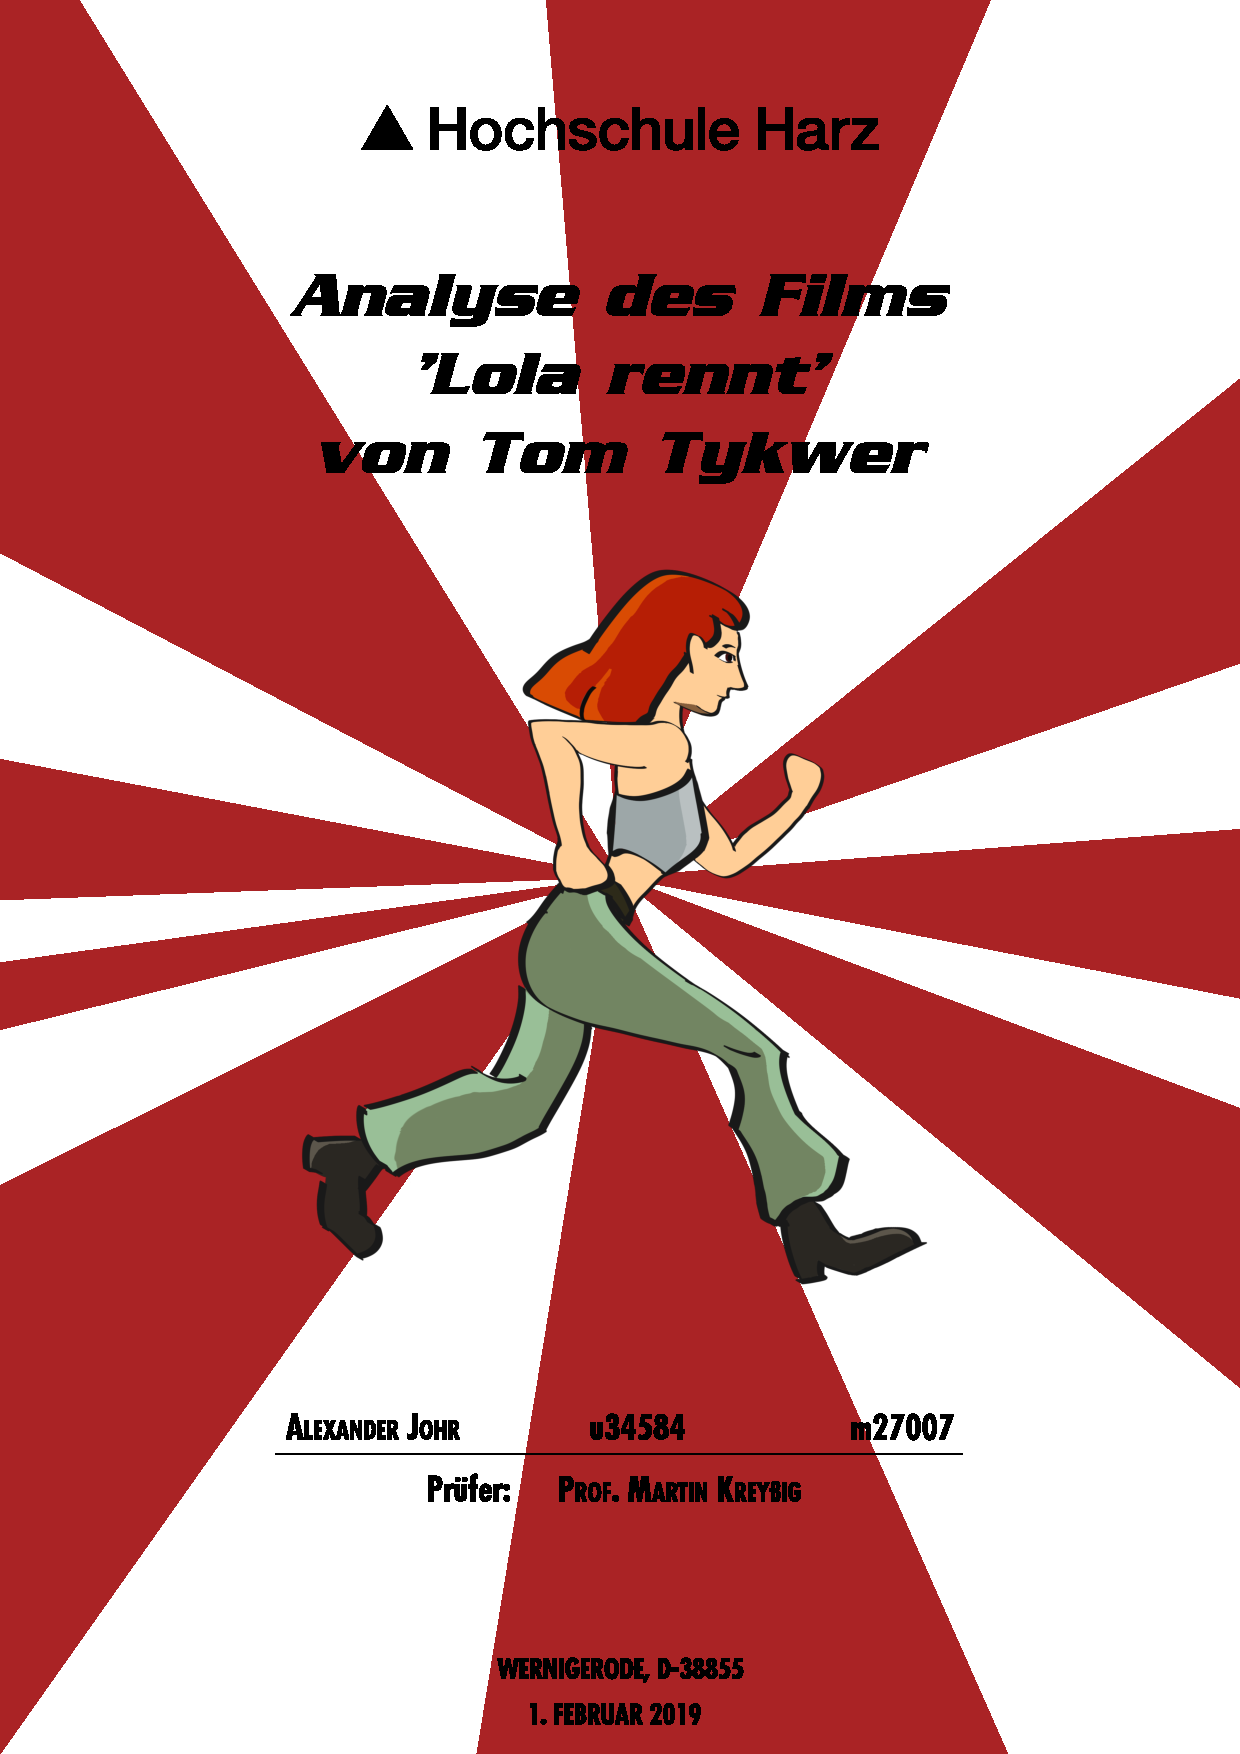
\includepdf[pages={1}]{FilmanalyseLolarenntDeckblatt.pdf}


\thispagestyle{plain}
\pagestyle{plain}

\tableofcontents

\listoffigures


\section{Analyse hinsichtlich der Zeit}

Bereits in der ersten Sequenz des Films 'Lola rennt' von Tom Tykwer wird der Zuschauer mit der Zeit konfrontiert. Zwei Zitate werden eingeblendet und greifen vor, dass es sich um Wiederholungen handeln wird: 

\begin{quote}
„Wir lassen nie vom Suchen ab, und doch, am Ende allen unseren Suchens, sind wir am Ausgangspunkt zurück und werden diesen Ort zum ersten Mal erfassen.“ (T.S. Eliot)
\par„Nach dem Spiel ist vor dem Spiel.“ (Sepp Herberger)
\end{quote}

Nach dem Verblassen der Zitate ertönt das Ticken einer Uhr. Ein Pendel schwenkt durch das Bild und kommt schließlich zum Stehen. Die Fratze eines Monsters wird sichtbar. Ein dramatischer Aufwärtsschwenk - begleitet durch unheimliche Technomusik - offenbart die verbundene Uhr, welche ebenfalls mit dämonischen Verzierungen versehen ist. Die sich überaus schnell drehenden Uhrzeiger und der schnelle Beat der Musik vermitteln das Gefühl von Zeitnot. Die intensivierten Geräusche von Pendel und Uhr sowie die dämonische Symbolik deuten an, dass etwas schreckliches passieren wird.

\subsection{Plot}

Lola und Manni sind ein Liebespaar wohnhaft in Berlin. Manni hat die Aufgabe als Geldkurier 100.000 Deutschen Mark um 12 Uhr zu seinem Auftraggeber, dem Gangsterboss Ronnie zu liefern. Manni ruft Lola nun an und bittet sie um Hilfe, da der Plan gehörig schief gegangen ist. Nach Erhalt der Tasche mit dem Geld war Lola nicht rechtzeitig am Treffpunkt, um Manni abzuholen, sodass er stattdessen die U-Bahn nehmen musste. Abgelenkt durch einen stolpernden Obdachlosen und durch in das Abteil eintretende Kontrolleure fühlt er sich reflexartig zur Flucht gezwungen und lässt dabei versehentlich die Tasche in der U-Bahn liegen. Es ist 11:40 Uhr und Lola hat etwa 20 Minuten sich eine Lösung zu überlegen. Außerdem muss sie zu Manni eilen, bevor dieser sich entschließt, das verloren gegangene Geld mit einem Überfall auf einen Supermarkt zu beschaffen.

\subsection{Zeitabschnitte}

Der experimentelle Charakter des Films wurde von Tom Tykwer nicht nur in der Handlung, sondern auch in der Auswahl der Stilmittel geprägt um, unter anderem, die Abgrenzung der Zeitabschnitte voneinander abzusetzen. Der Film startet mit der 35 mm Filmaufnahme und mit Mannis Anruf. Alle im Telefonat besprochenen vergangenen Ereignisse erscheinen in schwarz-weiß. Einige der Flashbacks beziehen sich auf denselben Tag, andere wiederum liegen in der unmittelbaren Vergangenheit, wie zum Beispiel Mannis Bestrafung durch Ronnie für die behaltene Zigarettenschachtel. Das Ende des Telefonats und der Flug des Telefonhörers durch die Luft leitet den Beginn der drei Läufe ein. Im Fernseher Lolas Mutter startet die Zweichentrick-Sequenz, welche für Tom Tykwer eine besondere Bedeutung hat: “Structurally speaking, the animation in the film is always the starting point for all domino principle type of changes in the causal chain.”.\footnote{\cite{AnythingRuns}}

Nach Verlassen des Hauses nimmt die Filmaufnahme wieder auf. Bei den Begegnungen mit den Nebencharakteren werden Vorgriffe auf die Zukunft dieser Charaktere eingeblendet. Zu diesem Zweck wird eine Fotoserie abgespielt, welche stets mit den Worten "`Und dann"' beginnt und von dem Ton einer auslösenden Kamera begleitet wird. Lola verpasst Manni, dieser beginnt pünktlich um 12 Uhr den Überfall und schließlich werden die beiden von der Polizei gestellt und Lola erschossen. Eine langsame Kamerafahrt auf ihr Gesicht und ein Abblenden in Rot startet einen weiteren Flashback. Nach der Aufblende bleibt die rote Färbung des Bildes bestehen. Rot wie das soeben vergossene Blut und gleichzeitig als Farbe der Liebe, welche auch als Gesprächsthema für Manni und Lola dient, während sie unbekleidet - zumindest im vom Close-Up sichtbaren Anschnitt - im Bett liegen. Die Aufnahme endet mit Lolas Worten "`Ich muss mich gerade entscheiden, glaub' ich."' Nach einem erneuten Abblenden in Rot und dem darauffolgenden Aufblenden sind wir zurück in der diegetischen Zeit. Lola nimmt nun das Syuzhet des Films selbst in die Hand. Sie sagt "`Stopp"` und plötzlich ist es wieder 11:40 Uhr und Lola wieder in ihrer Wohnung. Der zweite Lauf beginnt.

Erneut sind Flashforwards der Nebencharaktere zu sehen, nur dass sich diese von den vorherigen völlig unterscheiden. Dieses Mal erreicht Lola Manni rechtzeitig, doch er wird vom Krankenwagen überfahren. Ähnlich wie beim ersten Lauf setzt ein in Rot gefärbter Flashback ein. Nach dem Flashback beginnt der dritte und letzte Lauf.

%Nach Verlassen des Hauses nimmt die Filmaufnahme wieder auf. Bei den Begegnungen mit den Nebencharakteren werden bei jedem Lauf jeweils abweichende Vorgriffe auf die Zukunft dieser Charaktere eingeblendet. Zu diesem Zweck wird eine Fotoserie abgespielt, welche stets mit den Worten "`Und dann"' beginnt und von dem Ton einer auslösenden Kamera begleitet wird. Zwischen den drei Läufen werden weitere zwei Flashbacks eingespielt, in denen Manni und Lola unbekleidet - zumindest im vom Close-Up sichtbaren Anschnitt - im Bett liegen und sich unterhalten. Beide Aufnahmen sind in Rot gefärbt. Rot wie das soeben vergossene Blut und gleichzeitig als Farbe der Liebe, welches auch als Gesprächsthema dient. 

\subsection{Zeitangaben und Deutung}

Nach Lolas Schrei ist in einer Aufnahme in der Wohnung ein Altar mit Kerzen einer kleinen Statue und zwei Polaroid-Fotos zu sehen. Lola und Manni sind auf beiden Fotos abgebildet. Das Datum "`13.7.97"' ist auf einem der beiden Fotos notiert (Abb. \ref{fig:ManniUndLola}).

Auf der Bild-Zeitung, in der die Schlagzeile von Doris' Familie als Lotto-Gewinner abgedruckt ist, kann das Datum "`August 1997"' angeschnitten gefunden werden (Abb. \ref{fig:DorisZweiterFlashforward}, \ref{fig:DorisZweiterFlashforward2}). Auch in der alternativen Zukunft mit Doris als Mitglied von Jehovas Zeugen tauchen Ausgaben von "`Erwachet!"' und "`Der Wachtturm"' vom 15. und 22. August 1997 in ihrer Hand auf (Abb. \ref{fig:DorisDritterFlashforward}). \footnote{\cite{Rettung}} \footnote{\cite{DieWasserkriseEinWeltweitesProblem}} 
 
Die diegetische Zeit kann somit auf einen Tag zwischen dem 13.07.1997 und dem 15.08.97 eingeschränkt werden, sowie auf wenige Momente für die Dauer des Telefonates vor 11:40 Uhr bis wenige Augenblicke nach 12 Uhr, wie wiederholte Blicke auf Uhren verraten (Abb. \ref{fig:11Uhr40}, \ref{fig:12Uhr}).

Im ersten Lauf erfährt der Zuschauer während des Gesprächs zwischen Lola und ihrem Vater, dass sie mit Manni seit über einem Jahr zusammen ist. Somit können die rot gefärbten Szenen und damit die Fabula-Zeit bis 1996 zurückreichen.

Eine letzte Zeitangabe ist noch auf dem Herzfrequenzmessgerät in Form eines Aufklebers mit der Notiz "`23.5.98"' und einer Unterschrift zu finden (Abb. \ref{fig:Herzfrequenzmessgeraet}). Im Anbetracht der zuvor erwähnten Zeitdokumente kann dies als Datum der nächsten Prüfung des Gerätes gedeutet werden.

\subsection{Dominoeffekt und Chaostheorie}

Die außergewöhnliche Organisation des Films taucht wiederholt mit Referenzen in Form von Symbolen auf. Nach dem Telefonat mit Manni wirft Lola einen Blick auf den Fernseher. Dort ist eine Reihe an fallenden Dominosteinen zu beobachten. Eine Anspielung auf die Kettenreaktionen von Ereignissen, die den Verlauf der Handlung maßgeblich verändern.

Noch wesentlich häufiger tauchen Spiralen im Film auf. So ist etwa in der Zeichentrick-Sequenz, als Lola das Treppenhaus verlässt, eine Spirale im Türfenster erkennbar. Der Laden hinter der Telefonzelle, aus der Manni Lola anruft, trägt den Namen "`Spirale"' und ein Schild mit einer rotierenden Spirale ist an der Wand befestigt. Weitere Spiralen sind auf Lola und Mannis Kopfkissenbezügen zu finden. Die Chaostheorie beschreibt chaotische Systeme, in denen kleinste Änderungen am Startzustand gravierende Folgen für das Ergebnis mit sich bringen. Beispiele solcher Systeme, wie dem Lorenz- und dem Rössler-Attraktor werden in Form von Spiralen visualisiert. Alle Personen in 'Lola rennt' sind Akteure in einem solchen chaotischen System. Die Abweichungen der Ereignisse auf Lolas Weg scheinen zunächst unbedeutend zu sein. Mit der Zeit und dem Voranschreiten der Kettenreaktion ändert sich dies jedoch und entscheidet letztlich über Sieg oder Niederlage, Leben oder Tod.

\section{Zeitkonstruktion}

Der Artikel "`Zeitkonstruktion"' des Werks "`Filmanalyse"' beschäftigt sich mit der Frage, was die Zeitkonzeption mit der Filmanalyse zu tun hat.  \footnote{Vgl. \cite[S. 204]{keutzer2014filmanalyse}} Dieses Kapitel soll die getroffenen Aussagen über die Zeitkonstruktion mit dem Film 'Lola rennt' vergleichen bzw. ergänzen.

\subsection{Zeit als filmisches Motiv}
\label{lab:ZeitAlsFilmischesMotiv} 

'Lola rennt' ist ein experimenteller Film und zieht viele Parallelen zu einem Computerspiel.\footnote{\cite{AllesBlossEinSpiel}} Wie in einem Computerspiel üblich hat Lola mehrere Versuche. Sie wird befähigt, nach jeder Niederlage die Zeit zurückzudrehen. Doch nicht nur das, denn Lola lernt während dieser Versuche noch dazu, so zum Beispiel, wie man eine Pistole entsichert. Sie verfügt weiterhin über einen Glas zum Springen bringenden Schrei, mit dem sie auch das Raum-Zeit-Gefüge ihrem Willen beugt, um die Roulettekugel ein zweites Mal auf der 20 stehen bleiben zu lassen. Die Dauer der diegetischen Zeit von 20 Minuten wird dabei noch einmal thematisiert. 

\subsection{Die Dauer des Erzählens}

Die Hektik des Films wird mit Jump Cuts intensiviert. Nach dem Telefonat wirft Lola den Hörer in die Luft und denkt darüber nach, wer ihr helfen könnte. In einer schnellen Abfolge von Schnitten wird sie aus der gleichen Perspektive gezeigt. Die Position ihrer Hände am Kopf variiert dabei immer wieder. Der Telefonhörer landet exakt auf der Gabel des Apparats und verdeutlicht, dass in Wahrheit kaum Zeit vergangen ist. Es folgt die Trickblende, eingeleitet durch den Zeichentrick Croupier und seinen Worten "`ri­en ne va plus"'. Nun rotiert die Kamera um Lola und Jump Cuts zeigen unterschiedliche Personen, die sie in Gedanken durch geht. Geräusche einer rollenden Kugel und dem abschließenden Einlochen dieser unterstreichen das wiederkehrende Bild eines Roulette-Tischs.

Weitere Jump Cuts werden nach Lolas verlassen des Treppenhauses verwendet, wodurch der Film scheint vorgespult und Lola beschleunigt zu werden. Auch der Entschleunigung der sich langsam zu Boden bewegenden Besucher im Supermarkt während Mannis Überfall wird durch Jump Cuts entgegengewirkt:

\begin{quote}
Close-Up auf Manni: "`So, alle Kassen auf"' - Jump Cut - "`Die Kassen auf!"' - Over-shoulder shot - Close-Up auf Manni "`Kassen auf und hinlegen!"' - Jump Cut - "`Wer mich nervt, den knall' ich ab"' - Gegenschuss auf eine Besucherin - Close-Up auf Manni "`Wer mich nervt, den knall' ich ab"'.
\end{quote}

Nicht nur Jump Cuts zur Beschleunigung von Lola, sondern auch Zeitlupen werden während ihres Laufs eingesetzt. Insbesondere bei Überquerung der Brücke. Überblendungen deuten bereits an, dass sie auf dieser geradlinigen und ereignislose Strecke verhältnismäßig viel Zeit verbringt. Im Unterschied zu dem sonst sehr von Kurven und Hindernissen geprägten Weg hat sie hier Zeit nachzudenken. Zeit, die sie sich wünscht zu verlangsamen, um so schneller am Ziel anzukommen. Diesem Wunsch wird durch Zeitlupen Ausdruck verliehen. So auch in allen Szenen, in denen Lola ihr Ziel erreicht und hofft rechtzeitig zu sein. Während im Rest des Films mit Kreuzschnitt gearbeitet wird, finden hier Split Screens Anwendung, um die Gleichzeitigkeit der Ereignisse begreifbar zu machen. So etwa im ersten sowie zweiten Lauf - Lola kommt beim Supermarkt an. Über die gesamte Dauer des Split Screens, welcher Manni und Lola zeigt, wird eine Zeitlupe gelegt. Das Bild wird erneut geteilt und nun ist unter Manni und Lola noch die Uhr angeschnitten zu sehen. Lolas Schrei "`Manni!"' wurde dabei nicht durch eine Zeitlupe gezerrt, sondern in Normalgeschwindigkeit - jedoch verlängert - darüber gelegt und auch die Uhr ist nicht verlangsamt sondern in Wahrheit sogar beschleunigt, wie Filmeditorin Mathilde Bonnefoy verrät.  \footnote{\cite[S. 5]{DIEDRINGLICHKEITDERLIEBE}} 

Doch vor allem in den pathosgeladene Szenen finden Zeitlupen Anwendung. So zum Beispiel nach dem Überfall auf den Supermarkt. Der Sieg ist zum Greifen nah, aber auch die Angst nicht rechtzeitig zu entkommen begleitet die Flüchtigen. Eine von oben und unten zuschnappende Trickblende mit dem Geräusch einer ins Schloss fallenden Gefängnistür deutet bereits an, dass Lola und Manni der Polizei in die Falle gehen werden.  Der diegetische Ton setzt kurzweilig aus und die vergangenen Ereignisse werden durch Einsetzen des Songs 'What Difference A Day Makes' von Dinah Washington unterstrichen. Abwechselnd sind Ausschnitte mit und ohne Zeitlupe zu sehen, und ermöglichen dem Zuschauer das tatsächliche Tempo der Fluch fühlbar zu machen. Der diegetische Ton kehrt in Form der Sirenen  der Polizeiwagen zurück, welche Manni und Lola einkesseln. Die Zeitlupe setzt aus, um kurz darauf mit dem Schuss des Polizisten wieder einzusetzen und die nötige Dramatik zu schaffen. Dem Pathos wird erneut Ausdruck verliehen - durch beginnen melancholischer Musik, der Reduzierung des Tons auf die wesentlichen Geräusche und Verstärkung dieser (Der Knall der Pistole, Lolas stockende Atmung und der dumpfe Aufprall ihres Körpers, während sie zu Boden geht). 

\subsection{Die Ordnung des Erzählens}

\begin{quote}"'Chronologische Erzählungen mit einzelnen klar markierten Rückblenden finden sich in zahllosen Produktionen des klassischen Hollywoodkinos und bereiten in der Regel keinerlei Verständnisschwierigkeiten."`\footnote{\cite[S. 204]{keutzer2014filmanalyse}}\end{quote}
Gerade diese klare Markierung kann wie am Beispiel von 'Lola rennt' zu einer Herausforderung werden. Flashbacks werden durch die diegetische Sprache hinreichend erklärt und zusätzlich farblich kenntlich gemacht. Bei den Flashforwards musste darauf verzichtet werden. Um das Tempo des Films nicht zu stören, wurden die Polaroid-Sequenzen so eingespielt, sodass jedes Bild nur für eine Viertelsekunde sichtbar ist. Zu wenig Zeit, um den Zusammenhang zu erfassen, um auf Vergangenheit oder Zukunft zu deuten. Aus diesem Grund wurde die Entscheidung getroffen, durch eine Tafel mit den Worten "`Und dann"' eine weitere Markierung einzufügen.\footnote{Vgl. \cite[S. 7]{DIEDRINGLICHKEITDERLIEBE}} 

\subsection{Die Frequenz des Erzählens}

'Lola rennt' scheint auf den ersten Blick ein gutes Beispiel für das repetitive Erzählen zu sein:
\begin{quote}"`[...] üblich und
notwendig wird zumindest die partielle Repetition eines Zeitpunktes, wenn dieser als Ausgangs- oder Durchgangspunkt dient, von dem aus mehrere potentielle Varianten und Verläufe einer Erzählung entsponnen werden, wie es bei den gabelförmigen Erzählstrukturen
[...] der Fall ist"'\footnote{\cite[S. 216]{keutzer2014filmanalyse}}\end{quote}
Doch anders als beim angeführten Beispiel - dem Film "`Der Zufall möglicherweise"' - ist es Lola, die über den erneuten Versuch entscheidet. Die Zeit wird zurückgedreht, doch wie bereits in \ref{lab:ZeitAlsFilmischesMotiv} erwähnt, nimmt sie ihre Erfahrungen in die nächsten Versuche mit. Somit erscheint die Wiederholung eher wie eine Zeitreise und die Erzählung bekommt einen singulativen Charakter oder muss als Mischform aus singulativer und partiell repetitiver Erzählung gesehen werden.

\subsection{Schlussfolgerung}

Richtig ist, dass der Aspekt der Zeit in der Filmanalyse hohe Bedeutsamkeit innehat. Es liegt an der besonderen Art und Weise wie der Mensch die Zeit wahrnimmt. \footnote{Vgl. \cite[S. 204]{keutzer2014filmanalyse}} Im Film kann die Zeit mit unterschiedlichsten Hilfsmitteln manipuliert werden. Viele dieser Techniken sind dem Publikum bereits bekannt, da es die Raffung, Dehnung, Auslassung sowie Wiederholung der Zeit bereits an Träumen und Erinnerungen erfahren hat. Andere Techniken müssen genau markiert werden. Nicht zuletzt hat das Kino erprobt, wie weit es mit solchen Manipulationen gehen kann\footnote{Vgl. \cite[S. 216]{keutzer2014filmanalyse}}. Genau wegen dieses besonderen Blickes, den wir auf diese - doch eigentlich ganz gewöhnliche - physikalische Größe haben, ist die Konzeption der Zeit in der Analyse des Films so wichtig. Dies gilt ganz besonders für das für diese Analyse gewählte visuelles Feuerwerk namens 'Lola rennt'.


%\input{BaAJohrEinleitung}

%\input{BaAJohrQlikViewExtensions}

%\input{abstract}

%\setcounter{page}{1}




%\input{Alex}

%\input{Projektverlauf}

%\input{Meilensteine}
%\input{Pflichtenheft}
%\input{Projektplanung}
%\input{AnalyseTechnologien}


 

%\section{Module}
 
%\input{Module/Libov}
%\input{AnbindungDatenbanken}
%\input{Bluetooth}

%\input{Fachdatenbanken}

%\input{Shibboleth}

%\input{AnzeigeVoneBooks}

%\input{WidgetAnpassung}
%\input{Tastatur}
%\input{Lernsoftware}

%\input{Pong}
%\input{Merkzettel}

%\input{Radius}

%\input{RFID}
%\input{WIFIDirect}
%\input{WLANTriangolie}






%\input{CD}
%\input{UI}


%\input{SvnTuts}
\printbibliography[heading=bibintoc]

\appendix

\begin{appendix} 
\renewcommand{\thesubsection}{\Alph{subsection}}
\renewcommand\thefigure{\thesubsection.\arabic{figure}}   % figure caption A.1
\renewcommand\section{\stdsection}

\newpage

\section*{Anhang} 
\addcontentsline{toc}{section}{Anhang}%\addtocontents{toc}{\vfill}


\setcounter{figure}{0}    


\subsection{Filmausschnitte} 
\label{lab:Filmausschnitte}

\begin{figure}[htbp]
	\centering
		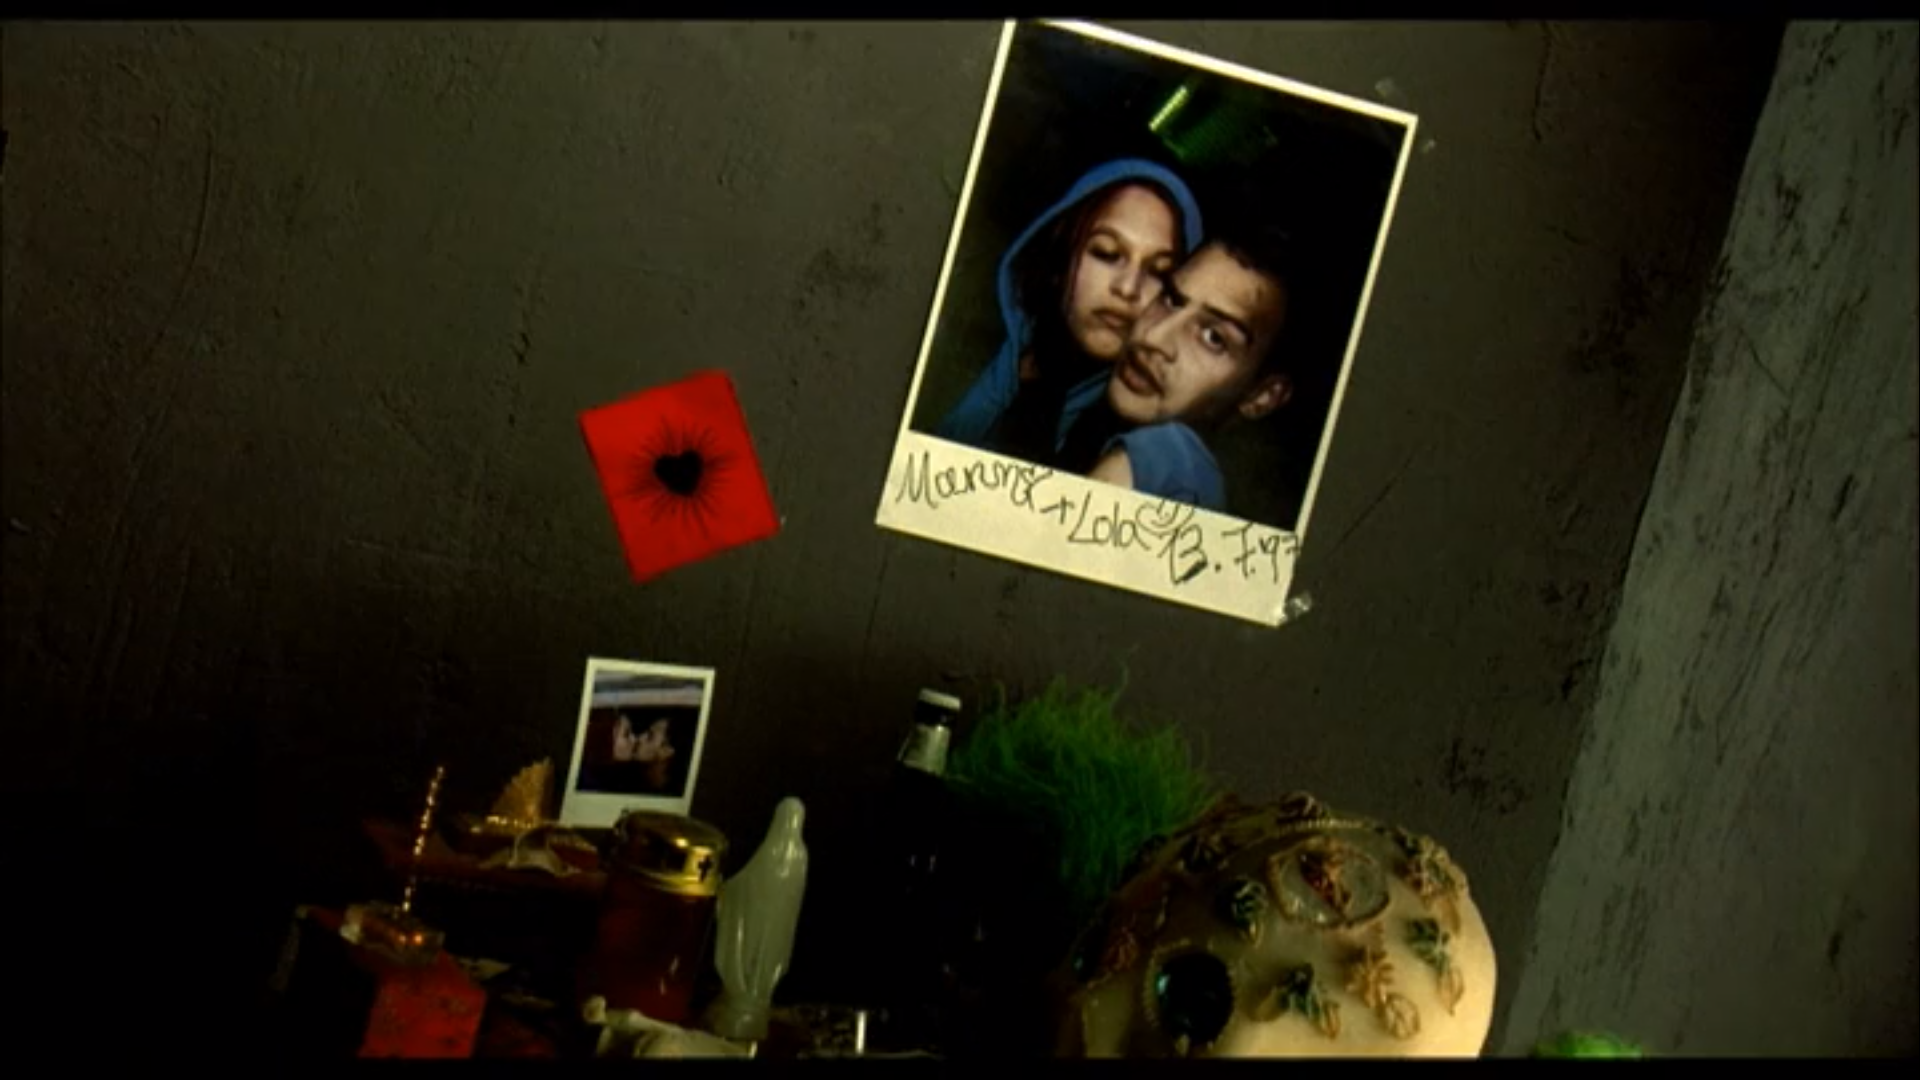
\includegraphics[width=1.00\textwidth]{img/ManniUndLola.png}
	\caption[Manni und Lola auf dem Polaroidfoto]{Manni und Lola auf dem Polaroidfoto \\Quelle: Lola rennt. Tom Tykwer. 1999. TC: 00:09:24}
	\label{fig:ManniUndLola}
\end{figure}

\begin{figure}[htbp]
	\centering
		\includegraphics[width=1.00\textwidth]{img/JackpotHerrlichkeit.png}
	\caption[Doris' zweiter Flashforward]{Doris' zweiter Flashforward \\Quelle: Lola rennt. Tom Tykwer. 1999. TC: 00:35:15}
	\label{fig:DorisZweiterFlashforward}
\end{figure}

\begin{figure}[htbp]
	\centering
		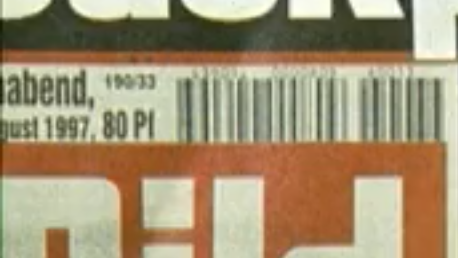
\includegraphics[width=0.69\textwidth]{img/JackpotHerrlichkeit2.png}
	\caption[Datum auf der Bild-Zeitung]{Datum auf der Bild-Zeitung \\Quelle: Lola rennt. Tom Tykwer. 1999. TC: 00:35:15}
	\label{fig:DorisZweiterFlashforward2}
\end{figure}

\begin{figure}[htbp]
	\centering
		\includegraphics[width=1.00\textwidth]{img/ZeugenJehovas.png}
	\caption[Doris' dritter Flashforward]{Doris' dritter Flashforward \\Quelle: Lola rennt. Tom Tykwer. 1999. TC: 00:53:59}
	\label{fig:DorisDritterFlashforward}
\end{figure}

\begin{figure}[htbp]
	\centering
		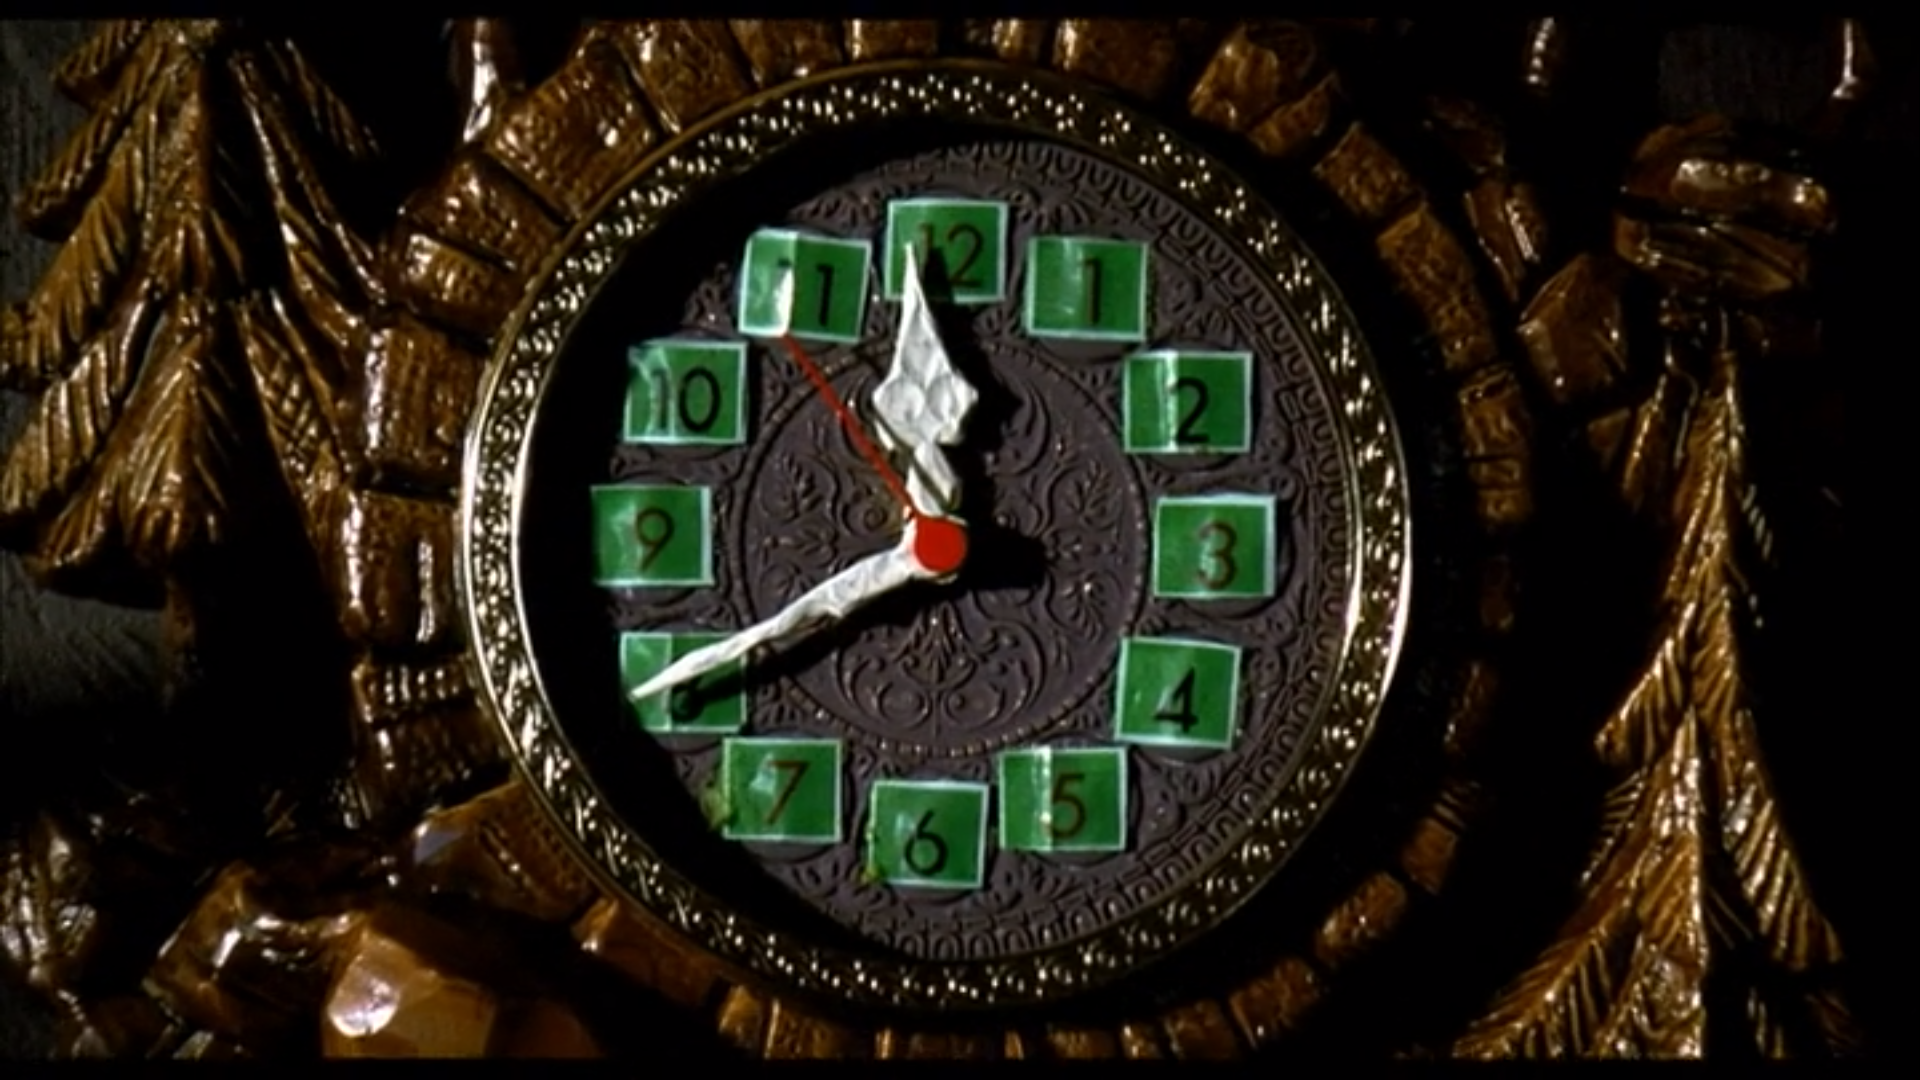
\includegraphics[width=1.00\textwidth]{img/11Uhr40.png}
	\caption[11:40 Uhr]{Lolas Blick auf die Uhr. Es ist 11 Uhr und 40 Minuten. \\Quelle: Lola rennt. Tom Tykwer. 1999. TC: 00:10:42}
	\label{fig:11Uhr40}
\end{figure}

\begin{figure}[htbp]
	\centering
		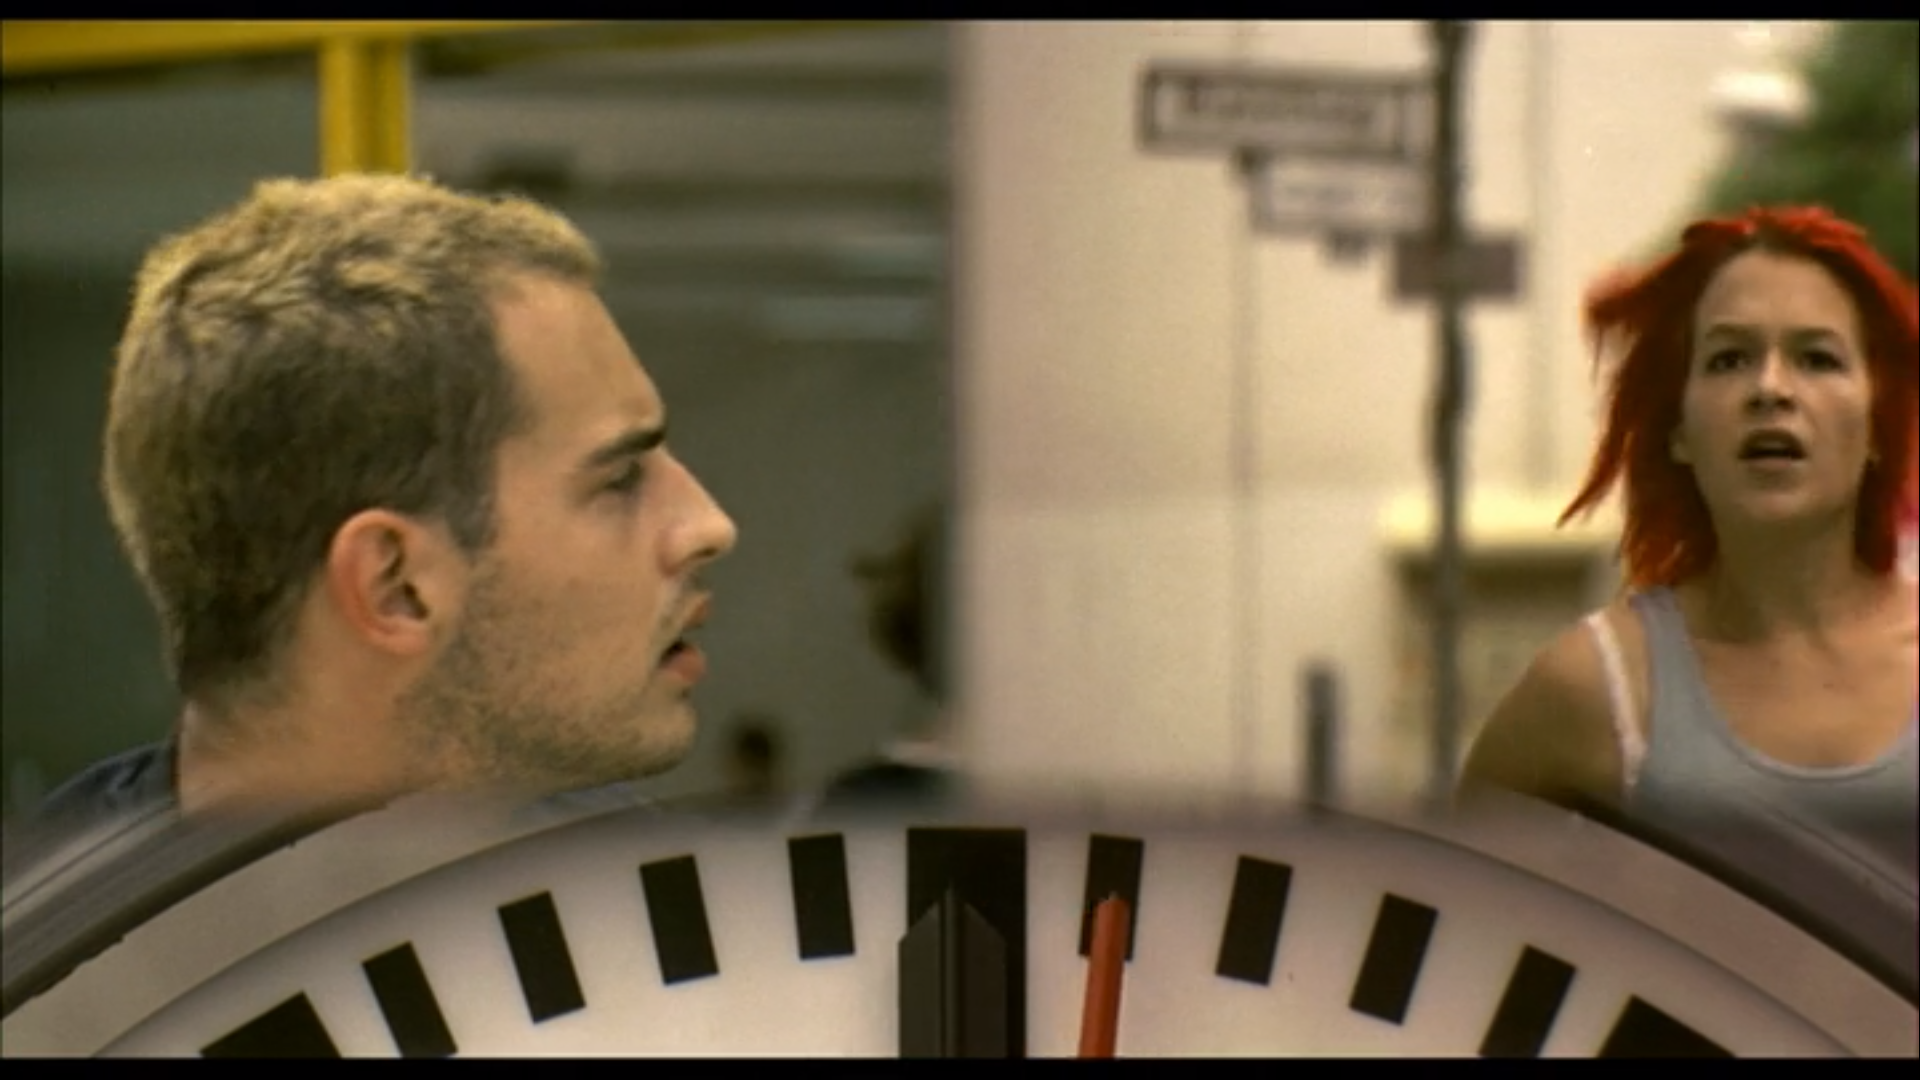
\includegraphics[width=1.00\textwidth]{img/12Uhr.png}
	\caption[12 Uhr]{Lola kann Manni rechtzeitig stoppen, den Supermarkt zu überfallen. Es ist 12 Uhr. \\Quelle: Lola rennt. Tom Tykwer. 1999. TC: 00:49:06}
	\label{fig:12Uhr}
\end{figure}

\begin{figure}[htbp]
	\centering
		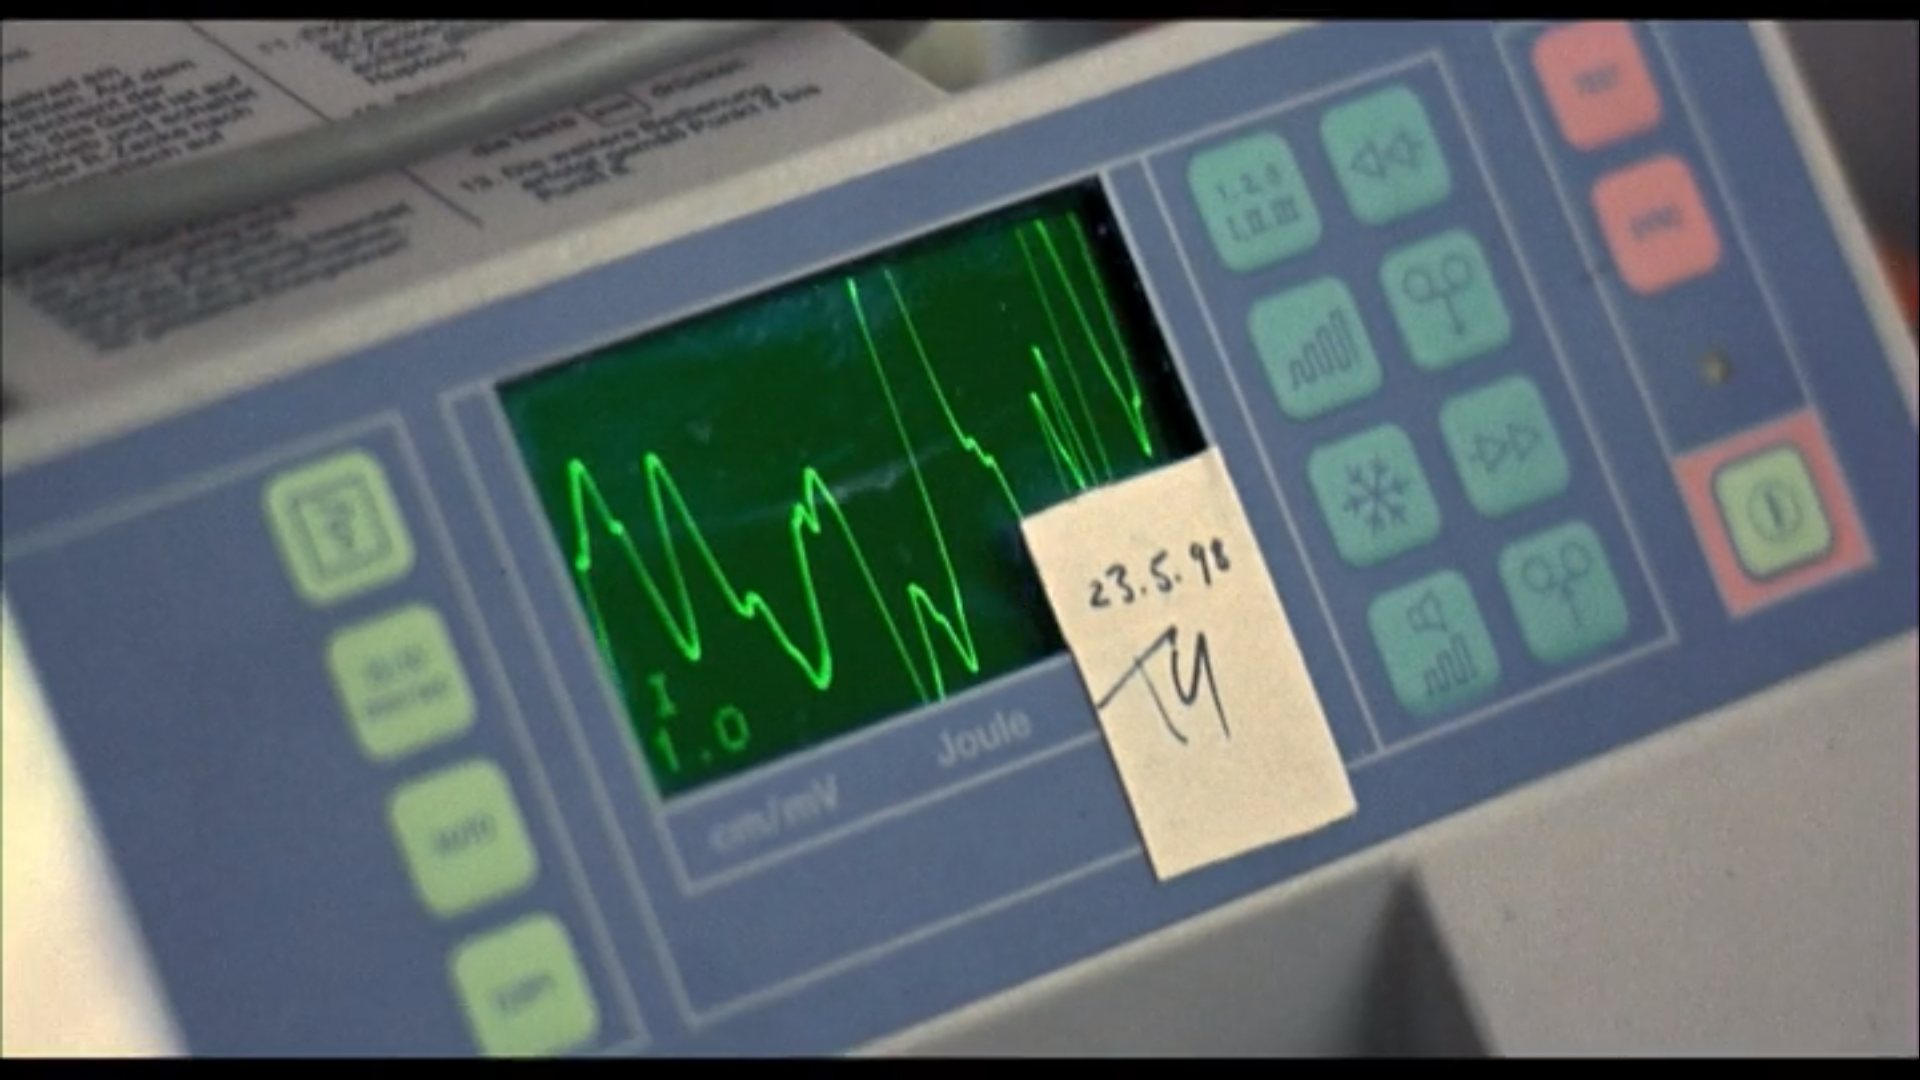
\includegraphics[width=1.00\textwidth]{img/Herzfrequenzmessgeraet.png}
	\caption[Das Herzfrequenzmessgerät]{Ein Aufkleber auf dem Herzfrequenzmessgerät mit der Notiz 23.5.98 und einer Unterschrift. \\Quelle: Lola rennt. Tom Tykwer. 1999. TC: 01:09:12}
	\label{fig:Herzfrequenzmessgeraet}
\end{figure}


\end{appendix} 


\mbox{}
\newpage




\setcounter{secnumdepth}{0} % Hide Section number in toc (If not: A Eidesstattliche Erklärung)

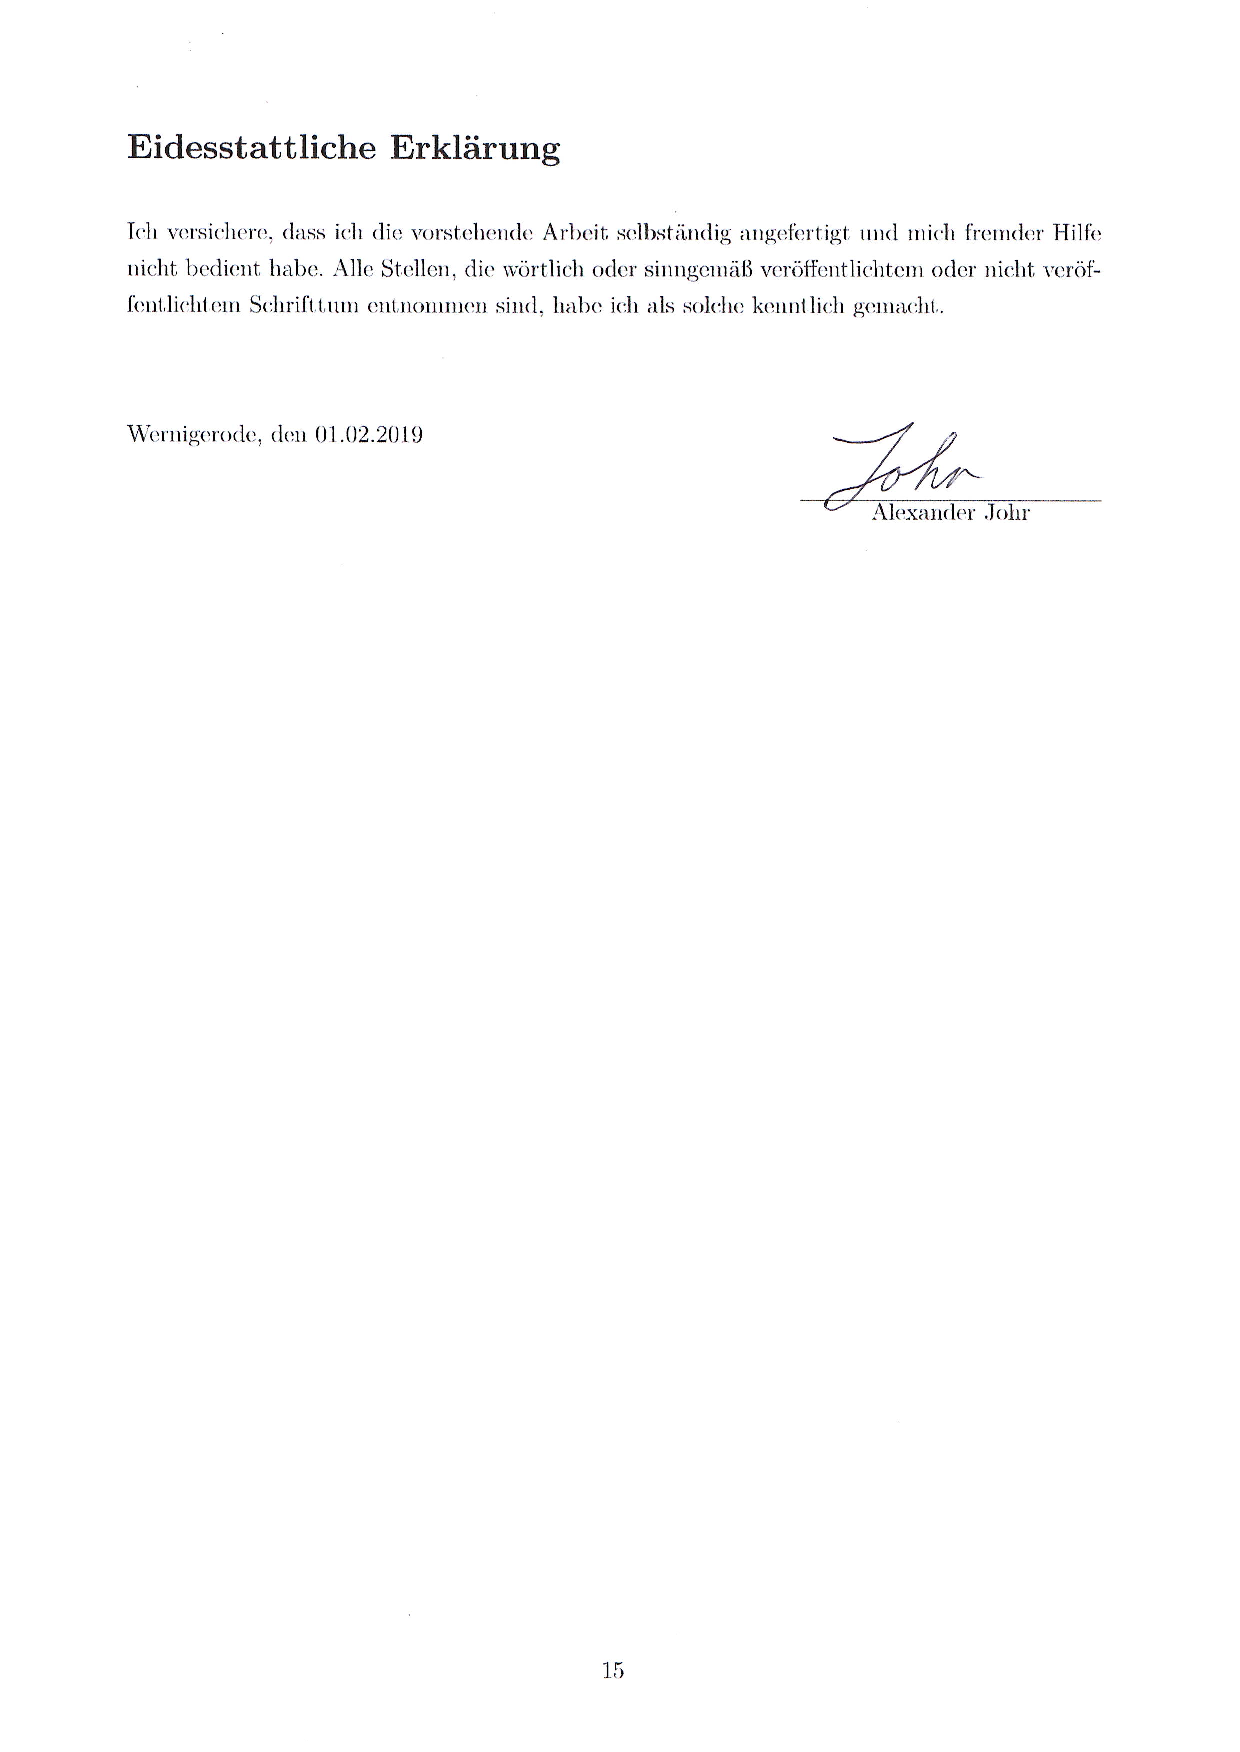
\includepdf[pages={1},addtotoc={
     1,section,1,Eidesstattliche Erkl\"arung,p1}]{EidesstattlicheErklaerung.pdf}

% Eidesstattliche Erklärung ununterschrieben
%\clearpage
%\section*{Eidesstattliche Erklärung}
%\addcontentsline{toc}{section}{Eidesstattliche Erklärung}%\addtocontents{toc}{\vfill}
%Ich versichere, dass ich die vorstehende Arbeit selbständig angefertigt und mich fremder Hilfe nicht bedient habe. Alle Stellen, die wörtlich oder sinngemäß veröffentlichtem oder nicht veröffentlichtem Schrifttum entnommen sind, habe ich als solche kenntlich gemacht.\\\\

%\noindent Wernigerode, den 01.02.2019
%\begin{flushright}
%$\overline{~~~~~~~~~\mbox{Alexander Johr}~~~~~~~~~}$
%\end{flushright}
%\mbox{}


\end{document}